% !TeX program = pdflatex
\documentclass[border=6pt]{standalone}
\usepackage{tikz}
\usetikzlibrary{arrows.meta, positioning, calc, fit, backgrounds}

\definecolor{MediumRed}{rgb}{0.925, 0.345, 0.345}
\definecolor{MediumGreen}{rgb}{0.37, 0.7, 0.66}
\definecolor{MediumBlue}{rgb}{0.015, 0.315, 0.45}
\definecolor{DarkBlue}{rgb}{0.05, 0.15, 0.35}

\begin{document}
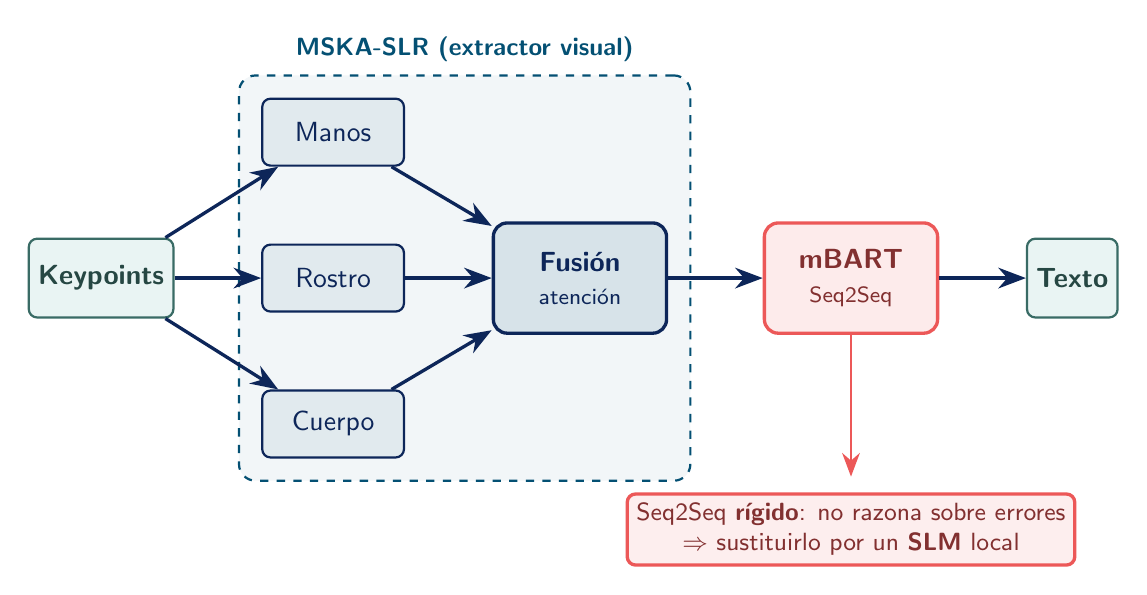
\begin{tikzpicture}[
    font=\sffamily,
    stream/.style={draw=DarkBlue, thick, rounded corners=3pt,
        fill=MediumBlue!12, text=DarkBlue, align=center,
        minimum width=1.8cm, minimum height=0.85cm},
    box/.style={draw=DarkBlue, very thick, rounded corners=5pt,
        fill=MediumBlue!16, text=DarkBlue, align=center,
        minimum width=2.2cm, minimum height=1.4cm},
    data/.style={draw=MediumGreen!60!black, thick, rounded corners=3pt,
        fill=MediumGreen!14, text=MediumGreen!40!black, align=center,
        minimum height=1.0cm},
    flow/.style={-{Stealth[length=3.5mm]}, line width=1.2pt, DarkBlue},
]

% entrada
\node[data] (kp) {\textbf{Keypoints}};

% tres flujos
\node[stream, above right=0.9cm and 1.1cm of kp] (s1) {Manos};
\node[stream, right=1.1cm of kp]                 (s2) {Rostro};
\node[stream, below right=0.9cm and 1.1cm of kp] (s3) {Cuerpo};
\foreach \s in {s1,s2,s3} \draw[flow] (kp)--(\s);

% fusion por atencion
\node[box, right=1.1cm of s2] (fus) {\textbf{Fusión}\\\footnotesize atención};
\foreach \s in {s1,s2,s3} \draw[flow] (\s)--(fus);

% decodificador
\node[box, right=1.2cm of fus, draw=MediumRed, fill=MediumRed!12,
      text=MediumRed!55!black] (mbart) {\textbf{mBART}\\\footnotesize Seq2Seq};
\draw[flow] (fus)--(mbart);

\node[data, right=1.1cm of mbart] (txt) {\textbf{Texto}};
\draw[flow] (mbart)--(txt);

% agrupar MSKA-SLR
\begin{scope}[on background layer]
    \node[draw=MediumBlue, dashed, thick, rounded corners=6pt,
          fill=MediumBlue!5, fit=(s1)(s3)(fus), inner sep=8pt] (mska) {};
\end{scope}
\node[font=\sffamily\small\bfseries, text=MediumBlue, above=1pt of mska.north]
    {MSKA-SLR (extractor visual)};

% el hueco
\node[draw=MediumRed, very thick, rounded corners=3pt, fill=MediumRed!10,
      text=MediumRed!55!black, font=\sffamily\small, align=center,
      below=2cm of mbart]
    {Seq2Seq \textbf{rígido}: no razona sobre errores\\
     $\Rightarrow$ sustituirlo por un \textbf{SLM} local};
\draw[-{Stealth[length=3mm]}, MediumRed, thick]
    ($(mbart.south)$) -- ++(0,-1.8);

\end{tikzpicture}
\end{document}
